\documentclass[final, table, cmyk]{beamer}
%% Possible paper sizes: a0, a0b, a1, a2, a3, a4.
%% Possible orientations: portrait, landscape
%% Font sizes can be changed using the scale option.
\usepackage[size=a0,orientation=portrait]{beamerposter}

\usepackage{euler}
% \usepackage[table]{xcolor}
\usetheme{gemini}
% \usecolortheme{seagull}

% ====================
% Packages
% ====================

\usepackage[utf8]{inputenc}
\usepackage{graphicx}
\usepackage{booktabs}
\usepackage{tikz}
\usepackage{pgfplots}

% ====================
% Lengths
% ====================

% If you have N columns, choose \sepwidth and \colwidth such that
% (N+1)*\sepwidth + N*\colwidth = \paperwidth
\newlength{\sepwidth}
\newlength{\colwidth}
\setlength{\sepwidth}{0.005\paperwidth}
\setlength{\colwidth}{0.48\paperwidth}

\newlength{\vboxsep}
\setlength{\vboxsep}{-.6\baselineskip}
\newlength{\mboxpreadjust}
\setlength{\mboxpreadjust}{-.4\baselineskip}

\newcommand{\separatorcolumn}{\begin{column}{\sepwidth}\end{column}}




%!TEX root = xprag-poster.tex

%% extra 

% colors

	\definecolor{maintheme}{cmyk}{.71, .51, 0, 0}
	\definecolor{highlight}{cmyk}{.05, .8, .05, 0}
	\definecolor{lowlight}{cmyk}{.64, .5, 0, .09}
	\definecolor{sechighlight}{cmyk}{0, .31, 100, .10}

	% \setbeamercolor{alerted text}{fg=orange}
	\setbeamercolor{background canvas}{bg=white}
	% \setbeamercolor{block body alerted}{bg=normal text.bg!90!black}
	\setbeamercolor{block body}{bg=normal text.bg!90!black}
	% \setbeamercolor{block body example}{bg=normal text.bg!90!black}
	% \setbeamercolor{block title alerted}{use={normal text,alerted text},fg=alerted text.fg!75!normal text.fg,bg=normal text.bg!75!black}
	% \setbeamercolor{block title}{bg=blue}
	% \setbeamercolor{block title example}{use={normal text,example text},fg=example text.fg!75!normal text.fg,bg=normal text.bg!75!black}
	% \setbeamercolor{fine separation line}{}
	% \setbeamercolor{frametitle}{fg=brown}
	% \setbeamercolor{item projected}{fg=black}
	\setbeamercolor{normal text}{fg=black}
	\setbeamercolor{caption name}{fg=black}
	% \setbeamercolor{separation line}{}
	\setbeamercolor{structure}{fg=maintheme}
	\setbeamercolor{title}{fg=maintheme, bg=lowlight}
	% \setbeamercolor{titlelike}{fg=maintheme}

	\definecolor{modal}{cmyk}{0, .31, 100, .0}
	\definecolor{cond}{cmyk}{.8, 0, .3, .3}
	\definecolor{neg}{cmyk}{.63, .23, 0, .0}
	\definecolor{question}{cmyk}{1, .36, 0, .30}

	\definecolor{red}{cmyk}{0,1,.5,0}

% boxes
	\usepackage{tcolorbox}
	\tcbuselibrary{skins}

	\newtcbox{\predhighlight}[1][lowlight]{on line,
	arc=3pt,colback=#1!10!white,colframe=#1!50!black,
	before upper={\rule[-3pt]{0pt}{10pt}},boxrule=1pt,
	boxsep=0pt,left=2pt,right=2pt,top=1pt,bottom=.5pt}

	\newtcbox{\ophighlight}[1][highlight]{on line,
	arc=3pt,colback=#1!10!white,colframe=#1!50!black,
	before upper={\rule[-3pt]{0pt}{10pt}},boxrule=1pt,
	boxsep=0pt,left=2pt,right=2pt,top=1pt,bottom=.5pt}

	\newtcolorbox{normalbox}[1]{colback=white,colframe=maintheme,fonttitle=\bfseries\Raleway\large,
	title={#1}}

	% \tcbset{colback=red!5!white,fonttitle=\bfseries}
	% \newtcolorbox{upshotbox}[1]{enhanced, squeezed title={#1}, frame style={left color=highlight, right color=lowlight!75!black}, leftrule=3mm, fonttitle=\bfseries\Raleway\Large, colback=highlight!5!white
	% }

	\newtcolorbox{upshotbox}[1]{
		colframe=highlight,
		colback=highlight!5!white,
		% colframe=maintheme,
		% colback=white,
		% coltitle=maintheme,
		adjusted title=center,halign title=center,
		title={#1},
		% frame style={left color=highlight, right color=lowlight!75!black},
		leftrule=3mm,
		fonttitle=\bfseries\Raleway\Large,
		%
		% detach title, before upper={\centering\tcbtitle\par}
	}

	\newtcolorbox{modelbox}[1]{
		% colback=lowlight!5!white,
		% colframe=lowlight,
		% coltitle=lowlight,
		colback=white,
		colframe=maintheme,
		coltitle=maintheme,
		text width=.95\linewidth,
		title={#1},
		fonttitle=\bfseries\footnotesize,
		detach title, before upper={\tcbtitle\par},
	}

	\newtcolorbox{theorybox}[1]{
		% colback=lowlight!5!white,
		% coltitle=lowlight,
		% colframe=lowlight,
		colback=white,
		colframe=maintheme,
		coltitle=maintheme,
		text width=.85\linewidth,
		title={#1},
		fonttitle=\bfseries\small,
		detach title, before upper={\tcbtitle\par},
	}

	\newtcolorbox{questionbox}[1]{
		colback=question!5!white,
		colframe=question,
		coltitle=question,
		% text width=.78\linewidth,
		title={#1},
		fonttitle=\bfseries,
		detach title, before upper={\tcbtitle},
	}

	\newtcolorbox{negbox}[1]{
		colback=neg!5!white,
		colframe=neg,
		coltitle=neg,
		% text width=.78\linewidth,
		title={#1},
		fonttitle=\bfseries,
		detach title, before upper={\tcbtitle},
	}

	\newtcolorbox{modalbox}[1]{
		colback=modal!5!white,
		colframe=modal,
		coltitle=modal,
		% text width=.78\linewidth,
		title={#1},
		fonttitle=\bfseries,
		detach title, before upper={\tcbtitle},
	}

	\newtcolorbox{condbox}[1]{
		colback=cond!5!white,
		colframe=cond,
		coltitle=cond,
		% text width=.78\linewidth,
		title={#1},
		fonttitle=\bfseries,
		detach title, before upper={\tcbtitle},
	}

	\newtcbox{\qhl}[1][lowlight]{on line,
	arc=3pt,colback=question!5!white,colframe=question,
	coltitle=question,
	before upper={\rule[-3pt]{0pt}{10pt}},boxrule=1pt,
	boxsep=0pt,left=2pt,right=2pt,top=1pt,bottom=.5pt}

	\newtcbox{\nhl}[1][lowlight]{on line,
	arc=3pt,colback=neg!5!white,colframe=neg,
	coltitle=neg,
	before upper={\rule[-3pt]{0pt}{10pt}},boxrule=1pt,
	boxsep=0pt,left=2pt,right=2pt,top=1pt,bottom=.5pt}

	\newtcbox{\mhl}[1][lowlight]{on line,
	arc=3pt,colback=modal!5!white,colframe=modal,
	coltitle=modal,
	before upper={\rule[-3pt]{0pt}{10pt}},boxrule=1pt,
	boxsep=0pt,left=2pt,right=2pt,top=1pt,bottom=.5pt}

	\newtcbox{\chl}[1][lowlight]{on line,
	arc=3pt,colback=cond!5!white,colframe=cond,
	coltitle=cond,
	before upper={\rule[-3pt]{0pt}{10pt}},boxrule=1pt,
	boxsep=0pt,left=2pt,right=2pt,top=1pt,bottom=.5pt}

% beamer elements
	% \useinnertheme{rounded}
	\setbeamertemplate{item}{\scriptsize$\blacktriangleright$}

% misc formatting
	\usepackage{linguex}
	\usepackage{booktabs}
	\usepackage[round]{natbib}
	\usepackage{multirow}
	\usepackage{rotating}

% drawing

	\usepackage{tikz}

% symbols 
	\usepackage{pifont}% http://ctan.org/pkg/pifont
	\newcommand{\cmark}{\ding{51}}%
	\newcommand{\xmark}{\ding{55}}%




%% Reference Sources
% \addbibresource{refs.bib}

\title{Projection variability of clausal complements across different operators}

\author{Lisa Hofmann\inst{1} \and Marie-Catherine de Marneffe\inst{2} \and Judith Tonhauser\inst{1}}

\institute[shortinst]{\inst{1} University of Stuttgart \samelineand \inst{2} UC Louvain}

\date{\today}

\begin{document}
	
\begin{frame}[t]

	\vspace{-2cm}
	\begin{columns}[t]
		\separatorcolumn
		
		\begin{column}{.74\colwidth}
			\begin{upshotbox}{Does the projection of content differ across entailment-canceling environments?}

				\begin{itemize}
					\item[\color{highlight}{$\blacktriangleright$}] \textbf{Yes!} Projection differs by entailment-cancelling \ophighlight{operator}
						
					\item[\color{highlight}{$\blacktriangleright$}] By-operator effects differ by predicate (\textbf{\ophighlight{operator}/\predhighlight{predicate} interaction})
					
					\item[\color{highlight}{$\blacktriangleright$}] Current theories of projective content do not predict our results
				\end{itemize}
				
			\end{upshotbox}
			\vspace{\vboxsep}
			\begin{normalbox}{Projection of clausal complements}
				Do you infer that Rachel is committed to the truth of the \textit{content of the complement} (CC), that \underline{\em Julian dances salsa}?
				
				\vspace{-.3\baselineskip}
				\ex. \a. Rachel: \emph{\lq Does Cole \predhighlight{know} that \underline{Julian dances salsa}?\rq}\\
					\cmark\ \  Yes, CC projects out of the question
					\b. Rachel: \emph{\lq Does Cole \predhighlight{think} that \underline{Julian dances salsa}?\rq}\\
					\xmark\ \ No, CC does not project
					\z.
				\z.
				
				\vspace{-.7\baselineskip}
				\resizebox{\linewidth}{!}{
					\begin{minipage}{1.7\linewidth}
						\citet{frege_uber_1892,strawson_referring_1950,kiparsky_fact_1970,karttunen_observations_1971,karttunen_conventional_1979}, and many more

					\end{minipage}
				}
			\end{normalbox}

			\vspace{\vboxsep}
			\begin{normalbox}{Entailment-cancelling operators}
				\textbf{Family-of-sentences test:}\newline No mention of differences in projection between different \ophighlight{operators}
				
				% \vspace{-.5\baselineskip}
				\ex. \phantom.\vspace{-2.8\baselineskip}\newline
					\begin{questionbox}{i. Polar question:}
						\hfill \textit{\ophighlight{Does} Cole know that Julian dances salsa?}
					\end{questionbox}
					\vspace{-.8\baselineskip}
					\begin{negbox}{ii. Negation:} \hfill \textit{Cole \ophighlight{doesn't} know that Julian dances salsa.}
					\end{negbox}
					\vspace{-.8\baselineskip}
					\begin{modalbox}{iii. Epistemic modal:}
						\hfill \textit{\ophighlight{Perhaps} Cole knows that Julian dances salsa.}
					\end{modalbox}
					\vspace{-.8\baselineskip}
					\begin{condbox}{iv. Conditional antecedents:}\newline
						\phantom.\hfill\textit{\ophighlight{If} Cole knows that Julian dances salsa, Logan will be joyful.}
					\end{condbox}
				\z.

				\vspace{-.5\baselineskip}
				\resizebox{\linewidth}{!}{
					\begin{minipage}{1.7\linewidth}
						(e.g. \citealt{chierchia_meaning_1990,coppock_invitation_2020})

					\end{minipage}
				}

			\end{normalbox}

			\vspace{\vboxsep}
			\begin{normalbox}{Hints at by-operator variation}
				% \hspace{-.02\linewidth}
					\begin{minipage}{1.08\linewidth}
						\begin{itemize}
							\item \citet{karttunen_observations_1971} proposes \textbf{factive vs semi-factive} distinction
							\item Smith \& Hall (\citeyear{smith_relationship_2014}): Experiment with \textbf{English projective contents}
							\begin{itemize}
								\item Effect of operator differs by projective content
							\end{itemize}
							\item Sieker \& Solstad (\citeyear{sieker_projective_2022}): Exp. with \textbf{German clause-embedding predicates}
							\begin{itemize}
								\item No by-predicate variation, no evidence for factive/semi-factive distinction
							\end{itemize}
						\end{itemize}
					\end{minipage}
				
				% \smallskip
				
				\begin{center}
					\scalebox{.85}{
					\begin{tabular}{l l c c c c}
					 	&& \nhl{\textcolor{neg}{\bf Neg}}  & \chl{\textcolor{cond}{\bf Cond}} &  \qhl{\textcolor{question}{\bf PQ}} & \mhl{\textcolor{modal}{\bf Mod}}  \\ \toprule

					 	&factives \\
					 	& \small (\textit{be annoyed, regret, \dots}) & 
					 		\multirow{-2}{*}{\cmark}	&
					 		\multirow{-2}{*}{\cmark}	&
					 		\multirow{-2}{*}{\cmark}	&
					 		\multirow{-2}{*}{\cmark}	\\

					 	 & semi-factives\\
					 	\multirow{-4}{*}{\parbox{2.5cm}{\footnotesize\centering \vspace{-\baselineskip}\phantom.\newline \citet{karttunen_observations_1971}}} &
					 	\small (\textit{discover, realize, see, notice, \dots}) & 
					 		\multirow{-2}{*}{\cmark}	&
					 		\multirow{-2}{*}{\parbox{2.5cm}{\footnotesize\centering \vspace{-\baselineskip}\phantom.\newline not\\ always}}	&
					 		\multirow{-2}{*}{\parbox{2.5cm}{\footnotesize\centering \vspace{-\baselineskip}\phantom.\newline not\\ always}}	&
					 		\multirow{-2}{*}{\parbox{2.5cm}{\footnotesize\centering \vspace{-\baselineskip}\phantom.\newline not\\ always}}	\\ \midrule

						& epithets (e.g. \textit{idiot}),
							&&& \cellcolor{gray!20} & \cellcolor{gray!20} \\
						& CC of \textit{know}&
					 		\multirow{-2}{*}{\parbox{2.5cm}{\footnotesize\centering \vspace{-.5\baselineskip}\phantom.\newline {\footnotesize\bf more}\\ projection}} &
					 		\multirow{-2}{*}{\parbox{2.5cm}{\footnotesize\centering \vspace{-.5\baselineskip}\phantom.\newline {\footnotesize\bf less}\\ projection}} &
					 		\cellcolor{gray!20}
					 		\multirow{-2}{*}{\parbox{2.5cm}{\footnotesize\centering \vspace{-.5\baselineskip}\phantom.\newline N/A}} &
					 		\cellcolor{gray!20}
					 		\multirow{-2}{*}{\parbox{2.5cm}{\footnotesize\centering \vspace{-.5\baselineskip}\phantom.\newline N/A}} \\

					 	& Appositive RCs,
							&&& \cellcolor{gray!20} & \cellcolor{gray!20} \\
						
						\multirow{-4}{*}{\parbox{3cm}{\footnotesize\centering \vspace{-\baselineskip}\phantom.\newline Smith \& Hall (\citeyear{smith_relationship_2014})}} &

						prep. content of \textit{win} &
					 		\multirow{-2}{*}{\parbox{2.5cm}{\footnotesize\centering \vspace{-.5\baselineskip}\phantom.\newline {\footnotesize\bf less}\\ projection}} &
					 		\multirow{-2}{*}{\parbox{2.5cm}{\footnotesize\centering \vspace{-.5\baselineskip}\phantom.\newline {\footnotesize\bf more}\\ projection}} &
					 		\cellcolor{gray!20}
					 		\multirow{-2}{*}{\parbox{2.5cm}{\footnotesize\centering \vspace{-.5\baselineskip}\phantom.\newline N/A}} &
					 		\cellcolor{gray!20}
					 		\multirow{-2}{*}{\parbox{2.5cm}{\footnotesize\centering \vspace{-.5\baselineskip}\phantom.\newline N/A}} \\ \midrule

					 	&CCs of German \lq factives\rq
							&&&&\\

						\multirow{-2}{*}{\parbox{3cm}{\footnotesize\centering \vspace{-\baselineskip}\phantom.\newline Sieker \& Solstad (\citeyear{sieker_projective_2022})}} &

						\& \lq semi-factives\rq&
					 		\multirow{-2}{*}{\parbox{2.5cm}{\footnotesize\centering \vspace{-.5\baselineskip}\phantom.\newline {\footnotesize\bf more}\\ projection}} &
					 		\multirow{-2}{*}{\parbox{2.5cm}{\footnotesize\centering \vspace{-.5\baselineskip}\phantom.\newline {\footnotesize\bf less}\\ projection}} &
					 		\multirow{-2}{*}{\parbox{2.5cm}{\footnotesize\centering \vspace{-.5\baselineskip}\phantom.\newline {\footnotesize\bf less}\\ projection}} &
					 		\multirow{-2}{*}{\parbox{2.5cm}{\footnotesize\centering \vspace{-.5\baselineskip}\phantom.\newline {\footnotesize\bf less}\\ projection}} \\ \bottomrule
					\end{tabular}}
				\end{center}
				
				
				% \vspace{-\baselineskip}

				\begin{figure}[h]
					\vspace{-.2\baselineskip}
					\centering
					\includegraphics[width=.7\linewidth]{sieker-solstad.png}
					\vspace{-.4\baselineskip}
					\caption{Sieker \& Solstad \citeyear{sieker_projective_2022}, p. 286: Projection-ratings by embedding operator, for purported factive and semi-factive predicates}
					% \label{fig:figure1}
				\end{figure}
				\vspace{-.8\baselineskip}
			\end{normalbox}

			\vspace{\vboxsep}
			\begin{normalbox}{\lq Certain-that\rq\ task for projection inferences}

				\begin{figure}[h]
					\centering
					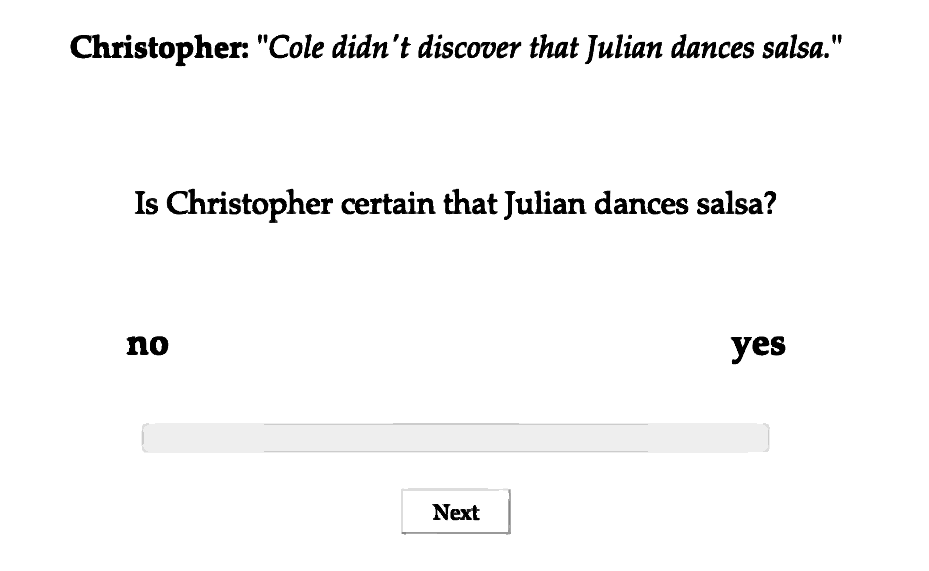
\includegraphics[width=.6\linewidth]{task-1n-proj.eps}
					% \caption{Caption here}
					\label{fig:task}
				\end{figure}

				\resizebox{\linewidth}{!}{
					\begin{minipage}{1.7\linewidth}
						\citet{tonhauser_prosodic_2016,djarv_prosodic_2017,tonhauser_how_2018,de_marneffe_commitmentbank_2019,mahler_social_2020,degen_are_2022,sieker_projective_2022}

					\end{minipage}
				}
				
			\end{normalbox}

			\vspace{\vboxsep}
			\begin{normalbox}{Variation among clause-embedding predicates}
				20 \predhighlight{predicates} that have shown projection variability in PQs\newline (\citealt{degen_are_2022})

				\begin{figure}[h]
					\centering
					\includegraphics[width=.95\linewidth]{degen-tonhauser.png}
					\vspace{-.8\baselineskip}
					\caption{\citealt{degen_are_2022}, p. 562: Mean certainty ratings by predicate}
					\label{fig:task}
				\end{figure}
				\vspace{-.8\baselineskip}
			\end{normalbox}

			\vspace{\vboxsep}
			\begin{normalbox}{Materials}
				To assess the effect of \ophighlight{operator} and \predhighlight{predicate} on \textbf{projection}:
				\vspace{.2\baselineskip}

					\textbf{4 experiments} (roughly $750$ participants each)
					\vspace{-.3\baselineskip}
					\begin{itemize}
						\item One per operator: \textcolor{question}{\bf polar questions}, \textcolor{neg}{\bf negation}, \textcolor{modal}{\bf modal \textit{perhaps}}, \textcolor{cond}{\bf conditional}
					\end{itemize}

					\vspace{-.2\baselineskip}
					Participants saw:
					\vspace{-.3\baselineskip}
					\begin{itemize}
						\item \textbf{20 clause embedding \predhighlight{predicates}}

						\begin{itemize}
							\item  Crossed with 20 CCs ($20 \times 20 = 400$ combinations)
						\end{itemize}

						\item (6 controls for exclusion)

					\end{itemize}
				\vspace{-.2\baselineskip}
				{\small (Experiments also used different at-issueness measures in separate block, not analyzed here)}

			\end{normalbox}
			
		\end{column}

		\separatorcolumn
		
		\begin{column}{1.25\colwidth}
			\begin{normalbox}{\phantom.\hfill Effects of operator \& predicate on projection}
				% \vspace{-\baselineskip}
				\hspace{-.2cm}\begin{tabular}{p{.70\linewidth} p{.3\linewidth}}
					\textcolor{highlight}{\large \Raleway \bfseries \underline{By-operator variation aggregating across predicates} (Figure 3)}
					\vspace{-.15\baselineskip}
					\begin{itemize} \small
						\item \chl{\textcolor{cond}{\bf Conditional}} > \qhl{\textcolor{question}{\bf Question}} > \nhl{\textcolor{neg}{\bf Negation}}, \mhl{\textcolor{modal}{\bf Modal}}
							\vspace{\mboxpreadjust}
							\begin{modelbox}{Model \#1: Linear mixed effect regression}
								\footnotesize
								response: \textbf{certainty ratings}; fixed effect: \ophighlight{operator} (base level: Question);
								random intercepts: participants, items; \newline
								MLEs: question (intercept) $0.51$, conditional $+0.05$, modal $-0.04$, negation $-0.03$; with all $p < 0.001$
							\end{modelbox}
							\vspace{\mboxpreadjust}

						\item But small differences, as in Sieker \& Solstad’s (2022) study
						\item Sieker \& Solstad’s results for German: Negation > Question, Conditional, Modal

					\end{itemize}

				\vspace{-.1\baselineskip}
				\textcolor{highlight}{\large \Raleway \bfseries\underline{Effect of operator differs by predicate} (Figure 4), e.g.}
				\vspace{-.15\baselineskip}
				\begin{itemize}\small
					\item CC of \predhighlight{be annoyed}: \qhl{\textcolor{question}{\bf Question}}, \nhl{\textcolor{neg}{\bf Negation}} > \chl{\textcolor{cond}{\bf Conditional}}, \mhl{\textcolor{modal}{\bf Modal}}
						\vspace{\mboxpreadjust}
						\begin{modelbox}{Model \#2: Linear mixed effect regression}
							\footnotesize
							response: \textbf{certainty ratings}; fixed effects: \ophighlight{operator}, \predhighlight{predicate}, and interaction (base lvl: \textbf{be annoyed} / negation); random intercepts: participant; 
							MLEs: negation (intercept) $0.87$, conditional $-0.12$, modal $-0.16$; ($p < 0.001$); question $+0.02$ (n.s.)
						\end{modelbox}

					\item CC of \predhighlight{know}: \qhl{\textcolor{question}{\bf Question}} > \nhl{\textcolor{neg}{\bf Negation}}, \chl{\textcolor{cond}{\bf Conditional}} > \mhl{\textcolor{modal}{\bf Modal}}
						\vspace{\mboxpreadjust}
						\begin{modelbox}{Model \#3: Linear mixed effect regression}
							\footnotesize
							response: \textbf{certainty ratings}; fixed effects: \ophighlight{operator}, \predhighlight{predicate}, and interaction (base level: \textbf{know} / negation); random intercepts: participant; \newline
							MLEs: negation (intercept) $0.79$, modal $-0.14$, question $+0.08$; with $p < 0.001$; , conditional $+/- 0$, (n.s.)
						\end{modelbox}

					\item CC of \predhighlight{discover}: \chl{\textcolor{cond}{\bf Conditional}}, \qhl{\textcolor{question}{\bf Question}} > \nhl{\textcolor{neg}{\bf Negation}} > \mhl{\textcolor{modal}{\bf Modal}}
						\vspace{\mboxpreadjust}
						\begin{modelbox}{Model \#4: Linear mixed effect regression}
							\footnotesize
							response: \textbf{certainty ratings}; fixed effects: \ophighlight{operator}, \predhighlight{predicate}, and interaction (base level: \textbf{discover} / negation); random intercepts: participant; \newline
							MLEs: negation (intercept) $0.68$, conditional $+0.11$, question $+0.10$, modal $-0.06$; with $p < 0.001$
						\end{modelbox}

				\end{itemize}

					&

					\vspace{-1.5\baselineskip}
						\begin{figure}[h]
							\resizebox{.85\linewidth}{!}{
							\centering
							\begin{tikzpicture}
							    \node at (0,0) {\includegraphics[width=.9\linewidth]{projective-op.pdf}};
							    % \draw[red,ultra thick,rounded corners] (7.5,5.3) rectangle (9.4,6.2);
							    \draw[highlight, ultra thick] (-3.37,2.3) -- (-3.37,1) -- node[below] {***} (-.66,1) -- (-.66,1.5);
							    \draw[highlight, ultra thick] (-.66,1.5) -- (-.66,.2) -- node[below] {***} (2.07,.2) -- (2.07,.7);
							    \draw[highlight, ultra thick] (2.07,.8) -- (2.07,.12) -- node[below] {\footnotesize n.s.} (4.78,.12) -- (4.78,.62);
							\end{tikzpicture}}
							\vspace{-1.4\baselineskip}
							\caption{Mean certainty ratings by operator}
							\label{fig:figure2}
						\end{figure}
					
				\end{tabular}
				\vspace{-1.24\baselineskip}
				\begin{figure}[h]
					\centering
					\includegraphics[width=\linewidth]{projective-pred-op.pdf}
					\vspace{-1.7\baselineskip}
					\caption{Mean certainty ratings by predicate with 95\% bootstrapped confidence intervals, grouped by operator. Entailment-cancelling operator coded by letter and color:  \textcolor{neg}{\texttt{N}: negation}, \textcolor{modal}{\texttt{M}: modals}, \textcolor{cond}{\texttt{C}: conditional antecedents}, \textcolor{question}{\texttt{Q}: polar questions}.
					}
					\label{fig:figure3}
				\end{figure}
				\vspace{-.8\baselineskip}
			\end{normalbox}
			
			\vspace{\vboxsep}
			\begin{normalbox}{\phantom.\hfill Discussion --- By-predicate variation in the effect of operator}
				\begin{itemize}
					\item Concurs with Smith \& Hall (\citeyear{smith_relationship_2014}), who found content/operator interactions for English projective contents
					\item Differs from Sieker \& Solstad (\citeyear{sieker_projective_2022}): found no predicate/operator interaction for CCs of German clause-embedding predicates
				\end{itemize}
				
				\textbf{No evidence for factive vs. semi-factive distinction (\citealt{karttunen_observations_1971})}
				\vspace{\mboxpreadjust}
				\begin{itemize}
					\item CC of purported factive \textit{be annoyed} does not invariably project across operators
					\item CC of purported semi-factives (\textit{discover, see}) do not project more across negation than other operators
				\end{itemize}

				\textbf{Provides support (from negation, modals, conditionals) for Degen \& Tonhauser’s (2022) result:}
				\vspace{\mboxpreadjust}
				\begin{itemize}
					\item Projection does not categorically differentiate between (semi-)factive/-factive predicates 
				\end{itemize}
				
			\end{normalbox}

			\vspace{\vboxsep}
			\begin{normalbox}{\phantom.\hfill Existing theories of projection do not predict our results}
				\centering
				\begin{theorybox}{Dynamic accounts of projection: Lexical triggering + dynamic semantics \hfill (\citealt{heim_presupposition_1992,van_der_sandt_presupposition_1992})}
					\small Distinguish factive and non-factive predicates:
					\vspace{-.3\baselineskip}
					\begin{itemize}
						\item \underline{factive} predicates (\textit{be annoyed, regret, \dots}): CC conventionally required to be contextually entailed in common ground
						\item \underline{non-factive} predicates (\textit{believe, say, …}): no such requirement
					\end{itemize}
					\vspace{-.2\baselineskip}
					Factive content projects globally, unless not admitted by common ground
				\end{theorybox}

				\begin{theorybox}{Lexical entailments + discourse-based triggering \hfill (\citealt{abrusan_predicting_2011,simons_best_2017})}
					\small Distinguish veridical predicates (CC is entailed) from non-veridical ones:
					\vspace{-.3\baselineskip}
					\begin{itemize}
						\item \underline{veridical} predicates (\textit{be right, demonstrate, \dots}): entailed CC projects if not at-issue
						\item \underline{non-veridical} predicates (\textit{believe, say, \dots}): no predictions / CC projects if required by discourse coherence
					\end{itemize}

				\end{theorybox}

				\begin{theorybox}{Contextual entailments + triggering based on cognitive inertness \hfill (\citealt{schlenker_triggering_2021})}
					\small Potential of projection for contents that are contextually entailed (given a context $C$ and the utterance $U$), including inferences from:
					\vspace{-.3\baselineskip}
					\begin{itemize}
						\item Lexically veridical predicates
						\item \lq Distributed veridicality\rq\ contexts (\citealt{roberts_i_2019}) \hfill (\textit{Cole \{was not wrong, can’t believe\} that Julian dances salsa.})
						\item Other sources of contextual inference \hfill ((Cole is honest + knowledgeable.) \textit{Cole said that Julian dances salsa.})
					\end{itemize}
					\vspace{-.2\baselineskip}
					Contextually entailed CC projects if it is an epistemic precondition of $U$ in $C$ (it is typically/likely already known).

				\end{theorybox}

				\smallskip
				\resizebox{\linewidth}{!}{
						\begin{tabular}{l c c c}
								& \multicolumn{3}{c}{\textbf{Predictions}}\\ \toprule
							%
							\textbf{Our data} 
								& \parbox{.3\linewidth}{\centering Lexical triggering + \par dynamic semantics}
									& \parbox{.3\linewidth}{\centering Lexical entailments +\par discourse-based triggering}
										& \parbox{.3\linewidth}{\centering Contextual entailments +\par triggering based on cognitive inertness} \\ \midrule
							%
							\parbox{.3\linewidth}{\raggedright\textbf{Superadditive predicate/operator interaction}\\[2.5\baselineskip]}
								& \parbox{.29\linewidth}{\centering \cellcolor{red!15} Meaning of entailment-canceling operators (invariably) encodes interaction with conventional content of embedded factives}
									& \parbox{.29\linewidth}{\centering \cellcolor{red!15} No systematic predictions for how veridicality or at-issueness interact with the meaning of entailment-canceling operators}
										& \parbox{.29\linewidth}{\centering\cellcolor{green!15} May be extended to our data by making explicit how combinations of operator + predicate are associated with contextual inferences}\\
							%
							\parbox{.3\linewidth}{\raggedright\textbf{Projection variability for all predicates}\par {\small Projection for some non-factive (/non-veridical) predicates as high as for some factive (/veridical) ones (see also D\&T'22)}\\[.5\baselineskip]}
								& \parbox{.29\linewidth}{\centering \cellcolor{red!15} No predictions for non-factive predicates}
									& \parbox{.29\linewidth}{\centering \cellcolor{red!15} No systematic predictions for non-veridical predicates}
										& \parbox{.29\linewidth}{\centering \cellcolor{green!15} Makes predictions about CCs of all clause-embedding predicates} \\
							%
							\parbox{.3\linewidth}{\raggedright\textbf{Out-of-the-blue contexts}\par {\small Projection variability in the out-of-the-blue contexts used in experiment (see also D\&T'22)}\\[1.7\baselineskip]}
								& \parbox{.29\linewidth}{\centering \cellcolor{red!15} Consistent projection of factive CCs}
									& \parbox{.3\linewidth}{\centering \cellcolor{green!15} Veridical predicates: analyses may be extended by assuming that the CCs of veridical predicates differ in at-issueness in out-of-the-blue contexts}
										& \parbox{.29\linewidth}{\centering \cellcolor{red!15} “Out-of-the-blue” contexts do not warrant assumption of contextual \underline{entailment}: No projection expected} \\
						\end{tabular}
				}

			\end{normalbox}

			\vspace{\vboxsep}
			\begin{upshotbox}{Theoretical implications}
				\begin{itemize}
					\item Previous work: projection analyses need to consider the effect of \textbf{lexical meaning} (e.g. \citealt{kiparsky_fact_1970,karttunen_observations_1971}, et. seq.), \textbf{world knowledge} (\citealt{de_marneffe_did_2012,degen_prior_2021}), and \textbf{discourse structure} (e.g. \citealt{simons_best_2017,tonhauser_how_2018})
					
					\item Add to that the effect of various \ophighlight{entailment-cancelling operators}
					
					\item An analysis of projection needs to be able to address \ophighlight{operator} / \predhighlight{predicate} interaction effects.

				\end{itemize}
			\end{upshotbox}

			\vspace{\vboxsep}
			\begin{normalbox}{\phantom.\hfill References}
				\tiny
				
				\textbf{M. Abrusán}. Predicting the presuppositions of soft triggers. \textit{L\&P}, 2011.\quad\textbullet\quad
				%
				\textbf{G. Chierchia and S. McConnell-Ginet.} \textit{Meaning and grammar: An introduction to semantics.} 1990.\quad\textbullet\quad
				%
				\textbf{E. Coppock and L. Champollion.} \textit{Invitation to formal semantics.} 2020.\quad\textbullet\quad
				%
				\textbf{M.-C. de Marneffe, M. Simons, and J. Tonhauser.} The CommitmentBank: Investigating projection in naturally occurring discourse. \textit{SuB}, 2019.\quad\textbullet\quad
				%
				\textbf{M.-C. de Marneffe, C.D. Manning, and C. Potts.} Did It Happen? The Pragmatic Complexity of Veridicality Assessment. \textit{Comp. Ling.}, February 2012.\quad\textbullet\quad
				%
				\textbf{J. Degen and J. Tonhauser.} Prior beliefs modulate projection. \textit{Open Mind}, 2021.\quad\textbullet\quad
				%
				\textbf{J. Degen and J. Tonhauser.} Are there factive predicates? An empirical investigation. \textit{Language}, 2022.\quad\textbullet\quad
				%
				\textbf{K. Djärv and H.A. Bacovcin.} Prosodic effects on factive presupposition projection. \textit{SALT}, 2017.\quad\textbullet\quad
				%
				\textbf{T. Roberts.} I can’t believe it’s not lexical: Deriving distributed veridicality. Semantics and Linguistic Theory, \textit{SALT}, 2019.\quad\textbullet\quad
				%
				\textbf{G. Frege.} Über Sinn und Bedeutung. \textit{Zeitschrift für Philosophie und philosophische Kritik}, 1892.\quad\textbullet\quad
				%
				\textbf{I. Heim.} Presupposition projection and the semantics of attitude verbs. \textit{JoS},1992.\quad\textbullet\quad
				%
				\textbf{L. Karttunen.} Some observations on factivity. \textit{Research on Language \& Social Interaction}, 1971.\quad\textbullet\quad
				%
				\textbf{L. Karttunen and S. Peters.} Conventional implicature. In Choon-Kyu Oh and David A. Dinneen, eds., \textit{Presuppositions, Syntax and Semantics}, 1979.\quad\textbullet\quad
				%
				\textbf{P. Kiparsky and C. Kiparsky.} Fact. In Manfred Bierwisch and Karl Erich Heidolph, eds., \textit{Progress in Linguistics}, 1970.\quad\textbullet\quad
				%
				\textbf{T. Mahler.} The social component of projection behavior of clausal complements. \textit{LSA}, 2020.\quad\textbullet\quad
				%
				\textbf{P. Schlenker.} Triggering presuppositions. \textit{Glossa}, 2021.\quad\textbullet\quad
				%
				\textbf{J. Sieker and T. Solstad.} Projective variability of (semi) factive verbs in family of sentence contexts: A rating study. \textit{AC 23}, 2022.\quad\textbullet\quad
				%
				\textbf{M. Simons, D. Beaver, C. Roberts, and J. Tonhauser.} The best question: Explaining the projection behavior of factives. \textit{Discourse processes}, 2017.\quad\textbullet\quad
				%
				\textbf{E.A. Smith and K.C. Hall.} The relationship between projection and embedding environment. \textit{CLS 48}. 2014.\quad\textbullet\quad
				%
				\textbf{P.F. Strawson.} On referring. \textit{Mind}, 1950.\quad\textbullet\quad
				%
				\textbf{J. Tonhauser.} Prosodic cues to presupposition projection. In \textit{SALT}, 2016.\quad\textbullet\quad
				%
				\textbf{J. Tonhauser, D.I. Beaver, and J. Degen.} How projective is projective content? Gradience in projectivity and at-issueness. \textit{JoS}, 2018.\quad\textbullet\quad
				%
				\textbf{R.A. v.d.Sandt.} Presupposition projection as anaphora resolution. \textit{JoS}, 1992.

			\end{normalbox}

			\vspace{20\baselineskip}
			\begin{normalbox}{References (not visible later)}
				\bibliographystyle{plainnat}
				\bibliography{projection}
			\end{normalbox}

		\end{column}
		\separatorcolumn
	\end{columns}



\end{frame}
\end{document}